\documentclass[twoside]{book}

% Packages required by doxygen
\usepackage{fixltx2e}
\usepackage{calc}
\usepackage{doxygen}
\usepackage[export]{adjustbox} % also loads graphicx
\usepackage{graphicx}
\usepackage[utf8]{inputenc}
\usepackage{makeidx}
\usepackage{multicol}
\usepackage{multirow}
\PassOptionsToPackage{warn}{textcomp}
\usepackage{textcomp}
\usepackage[nointegrals]{wasysym}
\usepackage[table]{xcolor}

% Font selection
\usepackage[T1]{fontenc}
\usepackage[scaled=.90]{helvet}
\usepackage{courier}
\usepackage{amssymb}
\usepackage{sectsty}
\renewcommand{\familydefault}{\sfdefault}
\allsectionsfont{%
  \fontseries{bc}\selectfont%
  \color{darkgray}%
}
\renewcommand{\DoxyLabelFont}{%
  \fontseries{bc}\selectfont%
  \color{darkgray}%
}
\newcommand{\+}{\discretionary{\mbox{\scriptsize$\hookleftarrow$}}{}{}}

% Page & text layout
\usepackage{geometry}
\geometry{%
  a4paper,%
  top=2.5cm,%
  bottom=2.5cm,%
  left=2.5cm,%
  right=2.5cm%
}
\tolerance=750
\hfuzz=15pt
\hbadness=750
\setlength{\emergencystretch}{15pt}
\setlength{\parindent}{0cm}
\setlength{\parskip}{3ex plus 2ex minus 2ex}
\makeatletter
\renewcommand{\paragraph}{%
  \@startsection{paragraph}{4}{0ex}{-1.0ex}{1.0ex}{%
    \normalfont\normalsize\bfseries\SS@parafont%
  }%
}
\renewcommand{\subparagraph}{%
  \@startsection{subparagraph}{5}{0ex}{-1.0ex}{1.0ex}{%
    \normalfont\normalsize\bfseries\SS@subparafont%
  }%
}
\makeatother

% Headers & footers
\usepackage{fancyhdr}
\pagestyle{fancyplain}
\fancyhead[LE]{\fancyplain{}{\bfseries\thepage}}
\fancyhead[CE]{\fancyplain{}{}}
\fancyhead[RE]{\fancyplain{}{\bfseries\leftmark}}
\fancyhead[LO]{\fancyplain{}{\bfseries\rightmark}}
\fancyhead[CO]{\fancyplain{}{}}
\fancyhead[RO]{\fancyplain{}{\bfseries\thepage}}
\fancyfoot[LE]{\fancyplain{}{}}
\fancyfoot[CE]{\fancyplain{}{}}
\fancyfoot[RE]{\fancyplain{}{\bfseries\scriptsize Generated by Doxygen }}
\fancyfoot[LO]{\fancyplain{}{\bfseries\scriptsize Generated by Doxygen }}
\fancyfoot[CO]{\fancyplain{}{}}
\fancyfoot[RO]{\fancyplain{}{}}
\renewcommand{\footrulewidth}{0.4pt}
\renewcommand{\chaptermark}[1]{%
  \markboth{#1}{}%
}
\renewcommand{\sectionmark}[1]{%
  \markright{\thesection\ #1}%
}

% Indices & bibliography
\usepackage{natbib}
\usepackage[titles]{tocloft}
\setcounter{tocdepth}{3}
\setcounter{secnumdepth}{5}
\makeindex

% Hyperlinks (required, but should be loaded last)
\usepackage{ifpdf}
\ifpdf
  \usepackage[pdftex,pagebackref=true]{hyperref}
\else
  \usepackage[ps2pdf,pagebackref=true]{hyperref}
\fi
\hypersetup{%
  colorlinks=true,%
  linkcolor=blue,%
  citecolor=blue,%
  unicode%
}

% Custom commands
\newcommand{\clearemptydoublepage}{%
  \newpage{\pagestyle{empty}\cleardoublepage}%
}

\usepackage{caption}
\captionsetup{labelsep=space,justification=centering,font={bf},singlelinecheck=off,skip=4pt,position=top}

%===== C O N T E N T S =====

\begin{document}

% Titlepage & ToC
\hypersetup{pageanchor=false,
             bookmarksnumbered=true,
             pdfencoding=unicode
            }
\pagenumbering{alph}
\begin{titlepage}
\vspace*{7cm}
\begin{center}%
{\Large My Project }\\
\vspace*{1cm}
{\large Generated by Doxygen 1.8.14}\\
\end{center}
\end{titlepage}
\clearemptydoublepage
\pagenumbering{roman}
\tableofcontents
\clearemptydoublepage
\pagenumbering{arabic}
\hypersetup{pageanchor=true}

%--- Begin generated contents ---
\chapter{Hierarchical Index}
\section{Class Hierarchy}
This inheritance list is sorted roughly, but not completely, alphabetically\+:\begin{DoxyCompactList}
\item I\+Pointer\+Enter\+Handler\begin{DoxyCompactList}
\item \contentsline{section}{do\+Exit}{\pageref{classdo_exit}}{}
\item \contentsline{section}{load\+Btn}{\pageref{classload_btn}}{}
\item \contentsline{section}{new\+Game}{\pageref{classnew_game}}{}
\end{DoxyCompactList}
\item I\+Pointer\+Exit\+Handler\begin{DoxyCompactList}
\item \contentsline{section}{do\+Exit}{\pageref{classdo_exit}}{}
\item \contentsline{section}{load\+Btn}{\pageref{classload_btn}}{}
\item \contentsline{section}{new\+Game}{\pageref{classnew_game}}{}
\end{DoxyCompactList}
\item \contentsline{section}{Main\+Player}{\pageref{class_main_player}}{}
\item \contentsline{section}{Main\+Rabbit}{\pageref{class_main_rabbit}}{}
\item \contentsline{section}{Main\+Wolf}{\pageref{class_main_wolf}}{}
\item Mono\+Behaviour\begin{DoxyCompactList}
\item \contentsline{section}{Bullet}{\pageref{class_bullet}}{}
\item \contentsline{section}{Bullet\+Script}{\pageref{class_bullet_script}}{}
\item \contentsline{section}{buttons}{\pageref{classbuttons}}{}
\item \contentsline{section}{camerafollow}{\pageref{classcamerafollow}}{}
\item \contentsline{section}{Character}{\pageref{class_character}}{}
\begin{DoxyCompactList}
\item \contentsline{section}{Enemy\+AI}{\pageref{class_enemy_a_i}}{}
\item \contentsline{section}{rabbit}{\pageref{classrabbit}}{}
\end{DoxyCompactList}
\item \contentsline{section}{do\+Exit}{\pageref{classdo_exit}}{}
\item \contentsline{section}{follow\+Background}{\pageref{classfollow_background}}{}
\item \contentsline{section}{generation\+Map}{\pageref{classgeneration_map}}{}
\item \contentsline{section}{load\+Btn}{\pageref{classload_btn}}{}
\item \contentsline{section}{Map\+Generate}{\pageref{class_map_generate}}{}
\item \contentsline{section}{New\+Behaviour\+Script}{\pageref{class_new_behaviour_script}}{}
\item \contentsline{section}{new\+Game}{\pageref{classnew_game}}{}
\item \contentsline{section}{Player}{\pageref{class_player}}{}
\item \contentsline{section}{Rabbit}{\pageref{class_rabbit}}{}
\item \contentsline{section}{range}{\pageref{classrange}}{}
\item \contentsline{section}{Range}{\pageref{class_range}}{}
\item \contentsline{section}{save\+Btn}{\pageref{classsave_btn}}{}
\item \contentsline{section}{Shooting}{\pageref{class_shooting}}{}
\item \contentsline{section}{Simply\+Player\+Behaviour}{\pageref{class_simply_player_behaviour}}{}
\item \contentsline{section}{Wolf}{\pageref{class_wolf}}{}
\item \contentsline{section}{Zdrowie\+UI}{\pageref{class_zdrowie_u_i}}{}
\end{DoxyCompactList}
\end{DoxyCompactList}

\chapter{Class Index}
\section{Class List}
Here are the classes, structs, unions and interfaces with brief descriptions\+:\begin{DoxyCompactList}
\item\contentsline{section}{\mbox{\hyperlink{class_bullet}{Bullet}} }{\pageref{class_bullet}}{}
\item\contentsline{section}{\mbox{\hyperlink{class_bullet_script}{Bullet\+Script}} }{\pageref{class_bullet_script}}{}
\item\contentsline{section}{\mbox{\hyperlink{classbuttons}{buttons}} }{\pageref{classbuttons}}{}
\item\contentsline{section}{\mbox{\hyperlink{classcamerafollow}{camerafollow}} }{\pageref{classcamerafollow}}{}
\item\contentsline{section}{\mbox{\hyperlink{class_character}{Character}} }{\pageref{class_character}}{}
\item\contentsline{section}{\mbox{\hyperlink{classdo_exit}{do\+Exit}} }{\pageref{classdo_exit}}{}
\item\contentsline{section}{\mbox{\hyperlink{class_enemy_a_i}{Enemy\+AI}} }{\pageref{class_enemy_a_i}}{}
\item\contentsline{section}{\mbox{\hyperlink{classfollow_background}{follow\+Background}} }{\pageref{classfollow_background}}{}
\item\contentsline{section}{\mbox{\hyperlink{classgeneration_map}{generation\+Map}} }{\pageref{classgeneration_map}}{}
\item\contentsline{section}{\mbox{\hyperlink{classload_btn}{load\+Btn}} }{\pageref{classload_btn}}{}
\item\contentsline{section}{\mbox{\hyperlink{class_main_player}{Main\+Player}} }{\pageref{class_main_player}}{}
\item\contentsline{section}{\mbox{\hyperlink{class_main_rabbit}{Main\+Rabbit}} }{\pageref{class_main_rabbit}}{}
\item\contentsline{section}{\mbox{\hyperlink{class_main_wolf}{Main\+Wolf}} }{\pageref{class_main_wolf}}{}
\item\contentsline{section}{\mbox{\hyperlink{class_map_generate}{Map\+Generate}} }{\pageref{class_map_generate}}{}
\item\contentsline{section}{\mbox{\hyperlink{class_new_behaviour_script}{New\+Behaviour\+Script}} }{\pageref{class_new_behaviour_script}}{}
\item\contentsline{section}{\mbox{\hyperlink{classnew_game}{new\+Game}} }{\pageref{classnew_game}}{}
\item\contentsline{section}{\mbox{\hyperlink{class_player}{Player}} }{\pageref{class_player}}{}
\item\contentsline{section}{\mbox{\hyperlink{class_rabbit}{Rabbit}} }{\pageref{class_rabbit}}{}
\item\contentsline{section}{\mbox{\hyperlink{classrabbit}{rabbit}} }{\pageref{classrabbit}}{}
\item\contentsline{section}{\mbox{\hyperlink{classrange}{range}} }{\pageref{classrange}}{}
\item\contentsline{section}{\mbox{\hyperlink{class_range}{Range}} }{\pageref{class_range}}{}
\item\contentsline{section}{\mbox{\hyperlink{classsave_btn}{save\+Btn}} }{\pageref{classsave_btn}}{}
\item\contentsline{section}{\mbox{\hyperlink{class_shooting}{Shooting}} }{\pageref{class_shooting}}{}
\item\contentsline{section}{\mbox{\hyperlink{class_simply_player_behaviour}{Simply\+Player\+Behaviour}} }{\pageref{class_simply_player_behaviour}}{}
\item\contentsline{section}{\mbox{\hyperlink{class_wolf}{Wolf}} }{\pageref{class_wolf}}{}
\item\contentsline{section}{\mbox{\hyperlink{class_zdrowie_u_i}{Zdrowie\+UI}} }{\pageref{class_zdrowie_u_i}}{}
\end{DoxyCompactList}

\chapter{Class Documentation}
\hypertarget{class_bullet}{}\section{Bullet Class Reference}
\label{class_bullet}\index{Bullet@{Bullet}}
Inheritance diagram for Bullet\+:\begin{figure}[H]
\begin{center}
\leavevmode
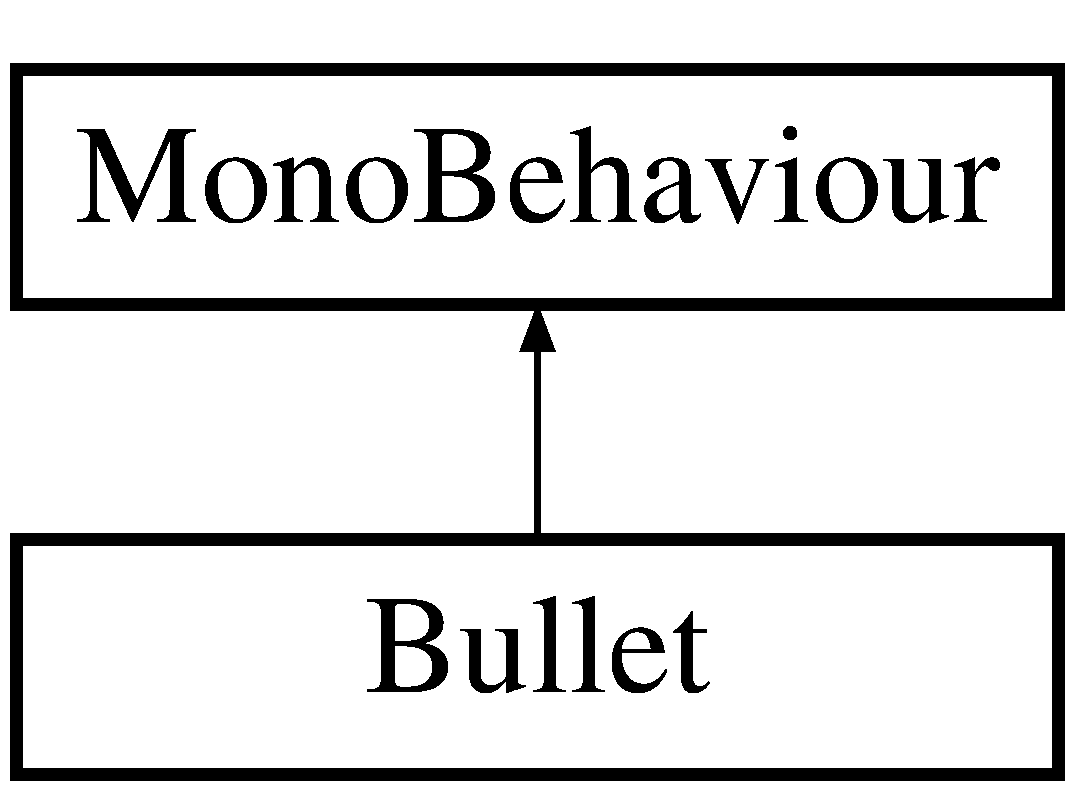
\includegraphics[height=2.000000cm]{class_bullet}
\end{center}
\end{figure}
\subsection*{Public Attributes}
\begin{DoxyCompactItemize}
\item 
\mbox{\Hypertarget{class_bullet_a0b778be60271e8555331383e78a7aa0f}\label{class_bullet_a0b778be60271e8555331383e78a7aa0f}} 
float {\bfseries velX} = 5f
\end{DoxyCompactItemize}


The documentation for this class was generated from the following file\+:\begin{DoxyCompactItemize}
\item 
Assets/Bullet.\+cs\end{DoxyCompactItemize}

\hypertarget{class_bullet_script}{}\section{Bullet\+Script Class Reference}
\label{class_bullet_script}\index{Bullet\+Script@{Bullet\+Script}}
Inheritance diagram for Bullet\+Script\+:\begin{figure}[H]
\begin{center}
\leavevmode
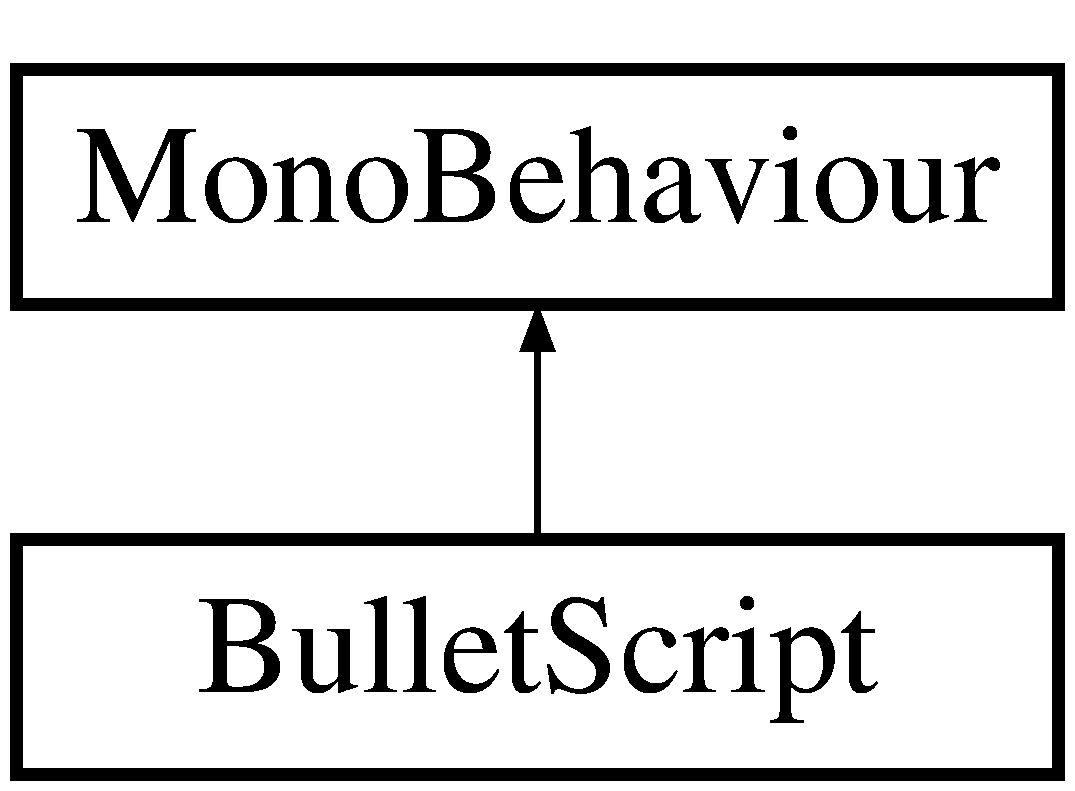
\includegraphics[height=2.000000cm]{class_bullet_script}
\end{center}
\end{figure}


The documentation for this class was generated from the following file\+:\begin{DoxyCompactItemize}
\item 
Assets/scripts/Bullet\+Script.\+cs\end{DoxyCompactItemize}

\hypertarget{classbuttons}{}\section{buttons Class Reference}
\label{classbuttons}\index{buttons@{buttons}}
Inheritance diagram for buttons\+:\begin{figure}[H]
\begin{center}
\leavevmode
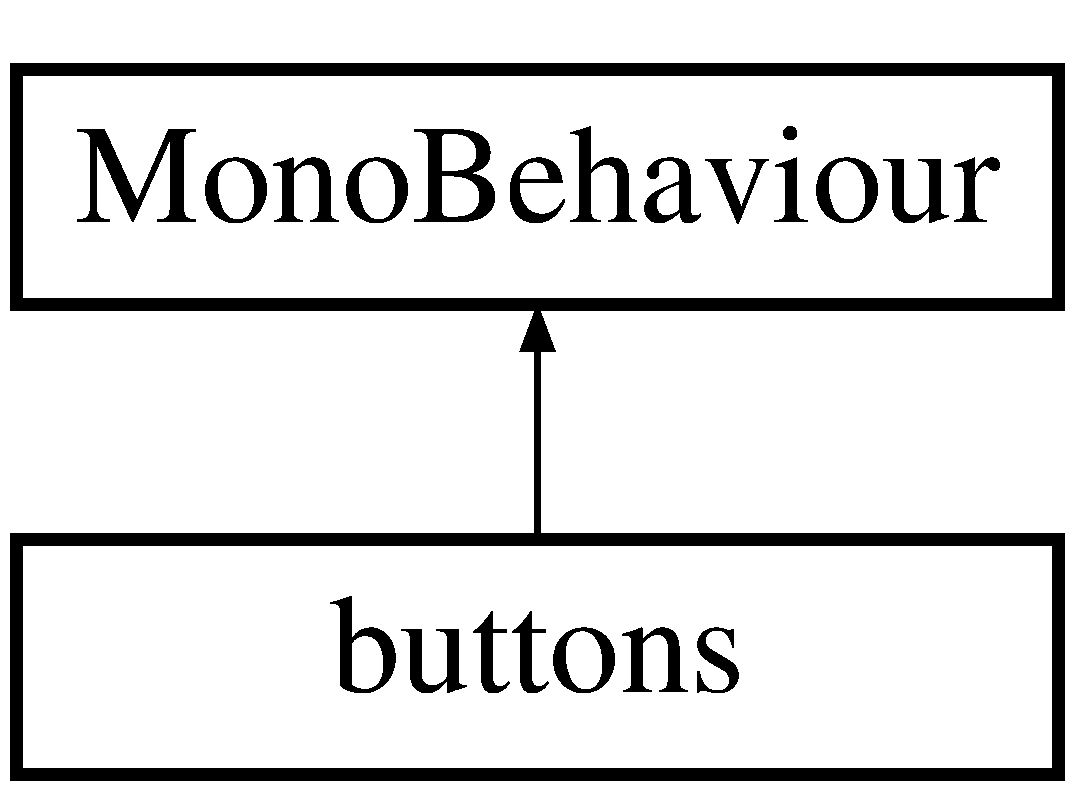
\includegraphics[height=2.000000cm]{classbuttons}
\end{center}
\end{figure}
\subsection*{Public Attributes}
\begin{DoxyCompactItemize}
\item 
\mbox{\Hypertarget{classbuttons_a0d09c922eebe4fb7476d96c915f3eb59}\label{classbuttons_a0d09c922eebe4fb7476d96c915f3eb59}} 
Texture {\bfseries btn\+Txt\+Exit}
\item 
\mbox{\Hypertarget{classbuttons_a1f3d953c197058e396bceb72a3488077}\label{classbuttons_a1f3d953c197058e396bceb72a3488077}} 
Texture {\bfseries btn\+Txt\+Save}
\item 
\mbox{\Hypertarget{classbuttons_a4013246c82d621dcde8250391386f1c0}\label{classbuttons_a4013246c82d621dcde8250391386f1c0}} 
Texture {\bfseries btn\+Txt\+To\+Menu}
\item 
\mbox{\Hypertarget{classbuttons_a09eeba1b6428f162c90e0037a49b54fc}\label{classbuttons_a09eeba1b6428f162c90e0037a49b54fc}} 
G\+U\+I\+Skin {\bfseries skin}
\end{DoxyCompactItemize}


The documentation for this class was generated from the following file\+:\begin{DoxyCompactItemize}
\item 
Assets/scripts/przyciski\+Podczas\+Gry/buttons.\+cs\end{DoxyCompactItemize}

\hypertarget{classcamerafollow}{}\section{camerafollow Class Reference}
\label{classcamerafollow}\index{camerafollow@{camerafollow}}
Inheritance diagram for camerafollow\+:\begin{figure}[H]
\begin{center}
\leavevmode
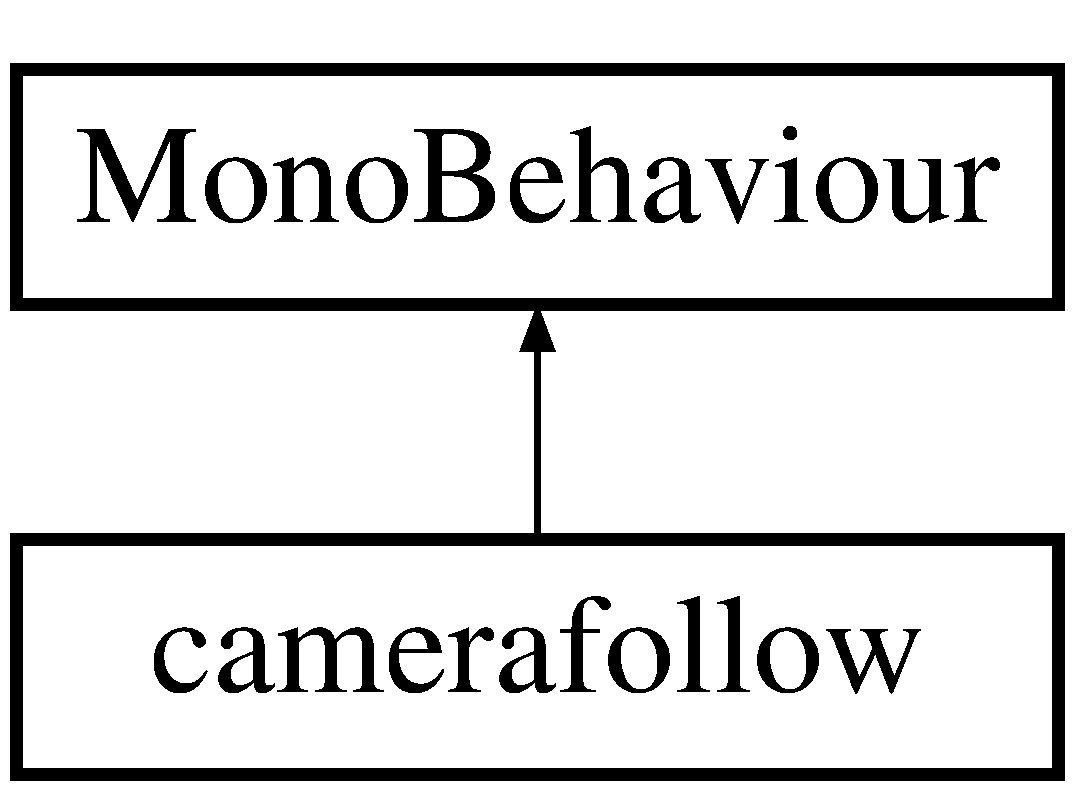
\includegraphics[height=2.000000cm]{classcamerafollow}
\end{center}
\end{figure}
\subsection*{Public Attributes}
\begin{DoxyCompactItemize}
\item 
\mbox{\Hypertarget{classcamerafollow_a688b31a08c146c63b6a0c07a6b917b01}\label{classcamerafollow_a688b31a08c146c63b6a0c07a6b917b01}} 
Game\+Object {\bfseries player}
\end{DoxyCompactItemize}


The documentation for this class was generated from the following file\+:\begin{DoxyCompactItemize}
\item 
Assets/back\+Ground\+Textures/camerafollow.\+cs\end{DoxyCompactItemize}

\hypertarget{class_character}{}\section{Character Class Reference}
\label{class_character}\index{Character@{Character}}
Inheritance diagram for Character\+:\begin{figure}[H]
\begin{center}
\leavevmode
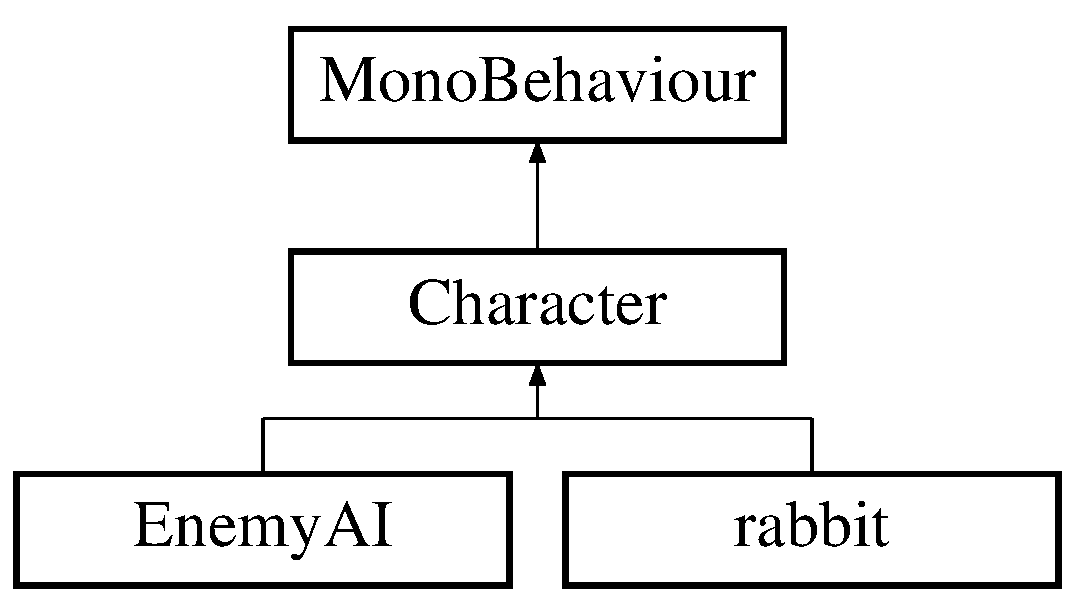
\includegraphics[height=3.000000cm]{class_character}
\end{center}
\end{figure}
\subsection*{Protected Attributes}
\begin{DoxyCompactItemize}
\item 
\mbox{\Hypertarget{class_character_aa86b30af2dd95e4208c38bd0810faac0}\label{class_character_aa86b30af2dd95e4208c38bd0810faac0}} 
Vector2 {\bfseries direction}
\end{DoxyCompactItemize}


The documentation for this class was generated from the following file\+:\begin{DoxyCompactItemize}
\item 
Assets/scripts/wolf/Character.\+cs\end{DoxyCompactItemize}

\hypertarget{classdo_exit}{}\section{do\+Exit Class Reference}
\label{classdo_exit}\index{do\+Exit@{do\+Exit}}
Inheritance diagram for do\+Exit\+:\begin{figure}[H]
\begin{center}
\leavevmode
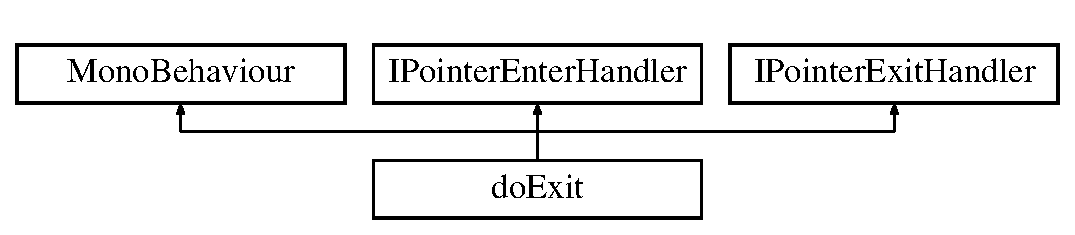
\includegraphics[height=2.000000cm]{classdo_exit}
\end{center}
\end{figure}
\subsection*{Public Member Functions}
\begin{DoxyCompactItemize}
\item 
\mbox{\Hypertarget{classdo_exit_a359569d05bd0a7182cf0715be4f9fece}\label{classdo_exit_a359569d05bd0a7182cf0715be4f9fece}} 
void {\bfseries do\+Quit} ()
\item 
\mbox{\Hypertarget{classdo_exit_ab09be60203d8a4919ef31d54726fb2bf}\label{classdo_exit_ab09be60203d8a4919ef31d54726fb2bf}} 
void {\bfseries On\+Pointer\+Enter} (Pointer\+Event\+Data event\+Data)
\item 
\mbox{\Hypertarget{classdo_exit_a81fe3192874bae06d0bcb2848c15d042}\label{classdo_exit_a81fe3192874bae06d0bcb2848c15d042}} 
void {\bfseries On\+Pointer\+Exit} (Pointer\+Event\+Data event\+Data)
\end{DoxyCompactItemize}
\subsection*{Public Attributes}
\begin{DoxyCompactItemize}
\item 
\mbox{\Hypertarget{classdo_exit_af4fddfa76423a0eb4e4d64a6d3a782e8}\label{classdo_exit_af4fddfa76423a0eb4e4d64a6d3a782e8}} 
Text {\bfseries the\+Text}
\end{DoxyCompactItemize}


The documentation for this class was generated from the following file\+:\begin{DoxyCompactItemize}
\item 
Assets/scripts/buttons\+Events/do\+Exit.\+cs\end{DoxyCompactItemize}

\hypertarget{class_enemy_a_i}{}\section{Enemy\+AI Class Reference}
\label{class_enemy_a_i}\index{Enemy\+AI@{Enemy\+AI}}
Inheritance diagram for Enemy\+AI\+:\begin{figure}[H]
\begin{center}
\leavevmode
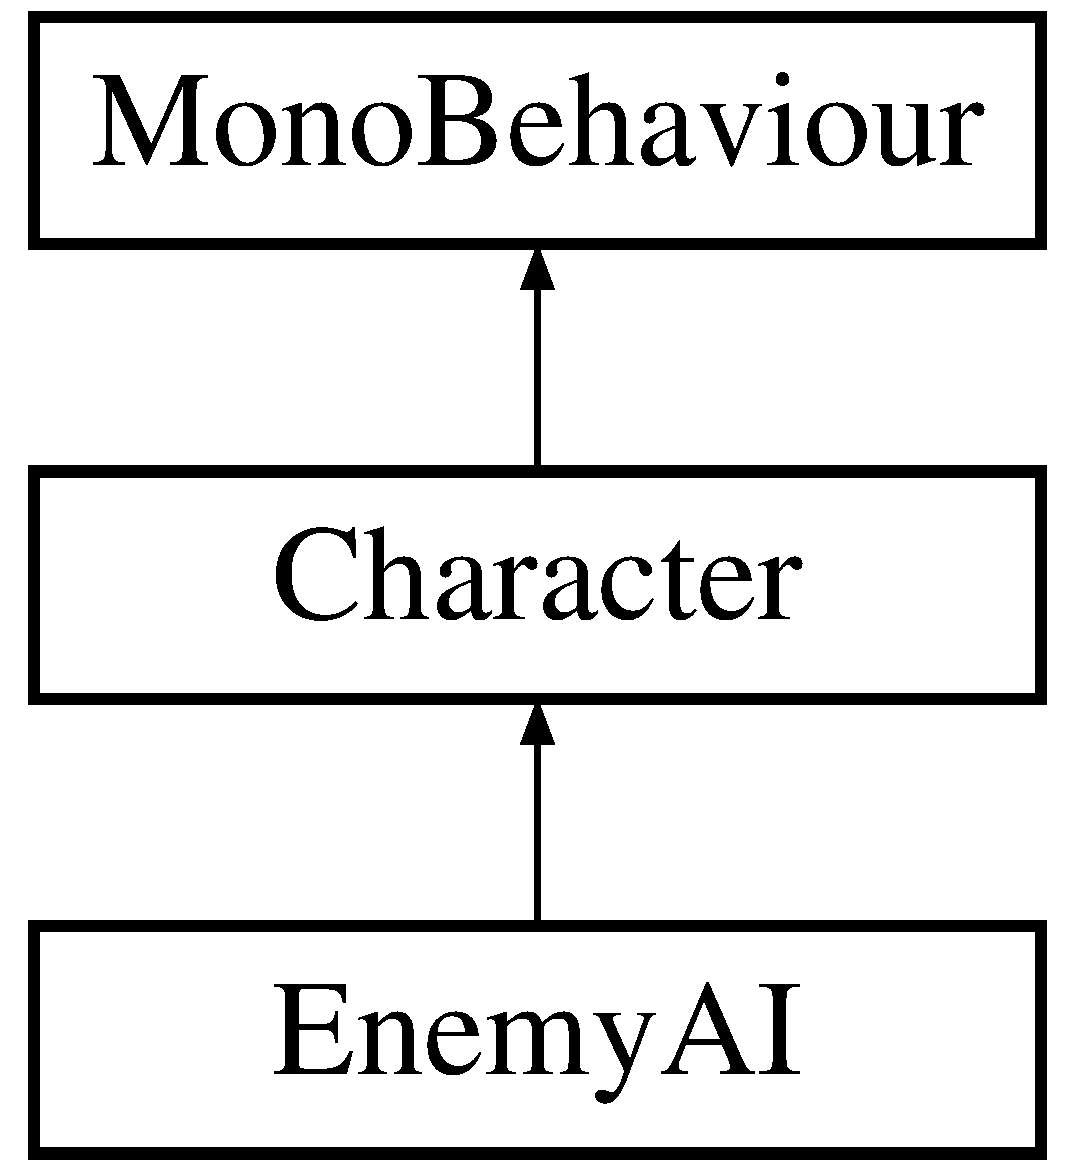
\includegraphics[height=3.000000cm]{class_enemy_a_i}
\end{center}
\end{figure}
\subsection*{Public Attributes}
\begin{DoxyCompactItemize}
\item 
\mbox{\Hypertarget{class_enemy_a_i_ae2f05a293142e35de08b31436e465c91}\label{class_enemy_a_i_ae2f05a293142e35de08b31436e465c91}} 
int {\bfseries move\+Speed}
\item 
\mbox{\Hypertarget{class_enemy_a_i_a33318434d46bd816d36c30b38ab17bc3}\label{class_enemy_a_i_a33318434d46bd816d36c30b38ab17bc3}} 
int {\bfseries rotation\+Speed}
\end{DoxyCompactItemize}
\subsection*{Properties}
\begin{DoxyCompactItemize}
\item 
\mbox{\Hypertarget{class_enemy_a_i_acdbde922eb7ccaabcf410b5051fcb241}\label{class_enemy_a_i_acdbde922eb7ccaabcf410b5051fcb241}} 
Transform {\bfseries Target}\hspace{0.3cm}{\ttfamily  \mbox{[}get, set\mbox{]}}
\end{DoxyCompactItemize}
\subsection*{Additional Inherited Members}


The documentation for this class was generated from the following file\+:\begin{DoxyCompactItemize}
\item 
Assets/scripts/wolf/Enemy\+A\+I.\+cs\end{DoxyCompactItemize}

\hypertarget{classfollow_background}{}\section{follow\+Background Class Reference}
\label{classfollow_background}\index{follow\+Background@{follow\+Background}}
Inheritance diagram for follow\+Background\+:\begin{figure}[H]
\begin{center}
\leavevmode
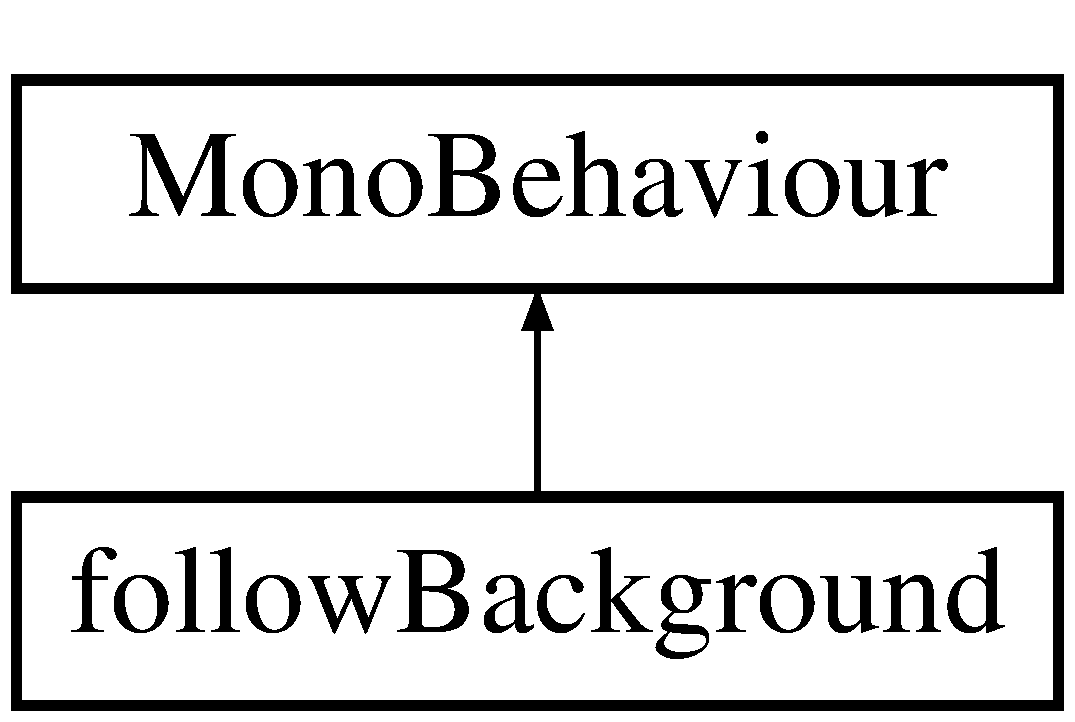
\includegraphics[height=2.000000cm]{classfollow_background}
\end{center}
\end{figure}


The documentation for this class was generated from the following file\+:\begin{DoxyCompactItemize}
\item 
Assets/scripts/bg\+Scripts/follow\+Background.\+cs\end{DoxyCompactItemize}

\hypertarget{classgeneration_map}{}\section{generation\+Map Class Reference}
\label{classgeneration_map}\index{generation\+Map@{generation\+Map}}
Inheritance diagram for generation\+Map\+:\begin{figure}[H]
\begin{center}
\leavevmode
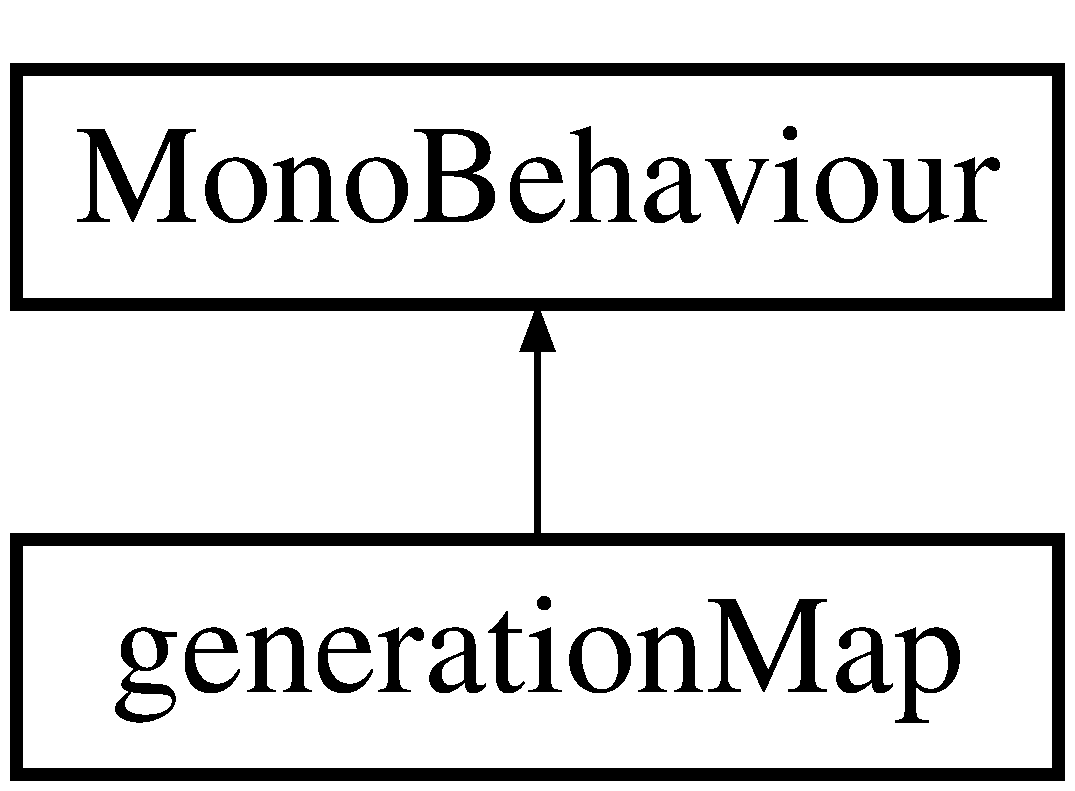
\includegraphics[height=2.000000cm]{classgeneration_map}
\end{center}
\end{figure}
\subsection*{Public Attributes}
\begin{DoxyCompactItemize}
\item 
\mbox{\Hypertarget{classgeneration_map_a3b44626f9ff72afdd6eb7b73bcf8fe34}\label{classgeneration_map_a3b44626f9ff72afdd6eb7b73bcf8fe34}} 
Game\+Object \mbox{[}$\,$\mbox{]} {\bfseries \+\_\+my\+Prefabs}
\end{DoxyCompactItemize}


The documentation for this class was generated from the following file\+:\begin{DoxyCompactItemize}
\item 
Assets/scripts/bg\+Scripts/generation\+Map.\+cs\end{DoxyCompactItemize}

\hypertarget{classload_btn}{}\section{load\+Btn Class Reference}
\label{classload_btn}\index{load\+Btn@{load\+Btn}}
Inheritance diagram for load\+Btn\+:\begin{figure}[H]
\begin{center}
\leavevmode
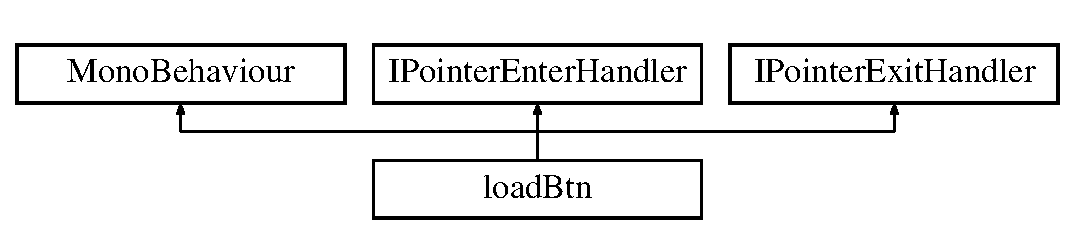
\includegraphics[height=2.000000cm]{classload_btn}
\end{center}
\end{figure}
\subsection*{Public Member Functions}
\begin{DoxyCompactItemize}
\item 
\mbox{\Hypertarget{classload_btn_a0fe1262f3fac6936b6c00f16e392537c}\label{classload_btn_a0fe1262f3fac6936b6c00f16e392537c}} 
void {\bfseries do\+Load} ()
\item 
\mbox{\Hypertarget{classload_btn_a04bdbf6ed6f0ce14b60d09d2173828db}\label{classload_btn_a04bdbf6ed6f0ce14b60d09d2173828db}} 
void {\bfseries On\+Pointer\+Enter} (Pointer\+Event\+Data event\+Data)
\item 
\mbox{\Hypertarget{classload_btn_a0c30fd768c3558cbac9f37557665c259}\label{classload_btn_a0c30fd768c3558cbac9f37557665c259}} 
void {\bfseries On\+Pointer\+Exit} (Pointer\+Event\+Data event\+Data)
\end{DoxyCompactItemize}
\subsection*{Public Attributes}
\begin{DoxyCompactItemize}
\item 
\mbox{\Hypertarget{classload_btn_a9ddffd0494944730e2ca5e43bffa6668}\label{classload_btn_a9ddffd0494944730e2ca5e43bffa6668}} 
Text {\bfseries the\+Text}
\end{DoxyCompactItemize}


The documentation for this class was generated from the following file\+:\begin{DoxyCompactItemize}
\item 
Assets/scripts/buttons\+Events/load\+Btn.\+cs\end{DoxyCompactItemize}

\hypertarget{class_main_player}{}\section{Main\+Player Class Reference}
\label{class_main_player}\index{Main\+Player@{Main\+Player}}
\subsection*{Properties}
\begin{DoxyCompactItemize}
\item 
\mbox{\Hypertarget{class_main_player_a40d6a53016917b2b7e5068a28656c2d7}\label{class_main_player_a40d6a53016917b2b7e5068a28656c2d7}} 
int {\bfseries Zdrowie}\hspace{0.3cm}{\ttfamily  \mbox{[}get, set\mbox{]}}
\item 
\mbox{\Hypertarget{class_main_player_a070928205b9aed8e06ab9db12784ed50}\label{class_main_player_a070928205b9aed8e06ab9db12784ed50}} 
int {\bfseries Glod}\hspace{0.3cm}{\ttfamily  \mbox{[}get, set\mbox{]}}
\item 
\mbox{\Hypertarget{class_main_player_aa3daa6c7d588f4020478fa6d701137db}\label{class_main_player_aa3daa6c7d588f4020478fa6d701137db}} 
int {\bfseries Woda}\hspace{0.3cm}{\ttfamily  \mbox{[}get, set\mbox{]}}
\end{DoxyCompactItemize}


The documentation for this class was generated from the following file\+:\begin{DoxyCompactItemize}
\item 
Assets/scripts/player/Main\+Player.\+cs\end{DoxyCompactItemize}

\hypertarget{class_main_rabbit}{}\section{Main\+Rabbit Class Reference}
\label{class_main_rabbit}\index{Main\+Rabbit@{Main\+Rabbit}}
\subsection*{Properties}
\begin{DoxyCompactItemize}
\item 
\mbox{\Hypertarget{class_main_rabbit_a2e479dd2b9ab6758a9da605d85dcfb4c}\label{class_main_rabbit_a2e479dd2b9ab6758a9da605d85dcfb4c}} 
int {\bfseries Zdrowie}\hspace{0.3cm}{\ttfamily  \mbox{[}get, set\mbox{]}}
\end{DoxyCompactItemize}


The documentation for this class was generated from the following file\+:\begin{DoxyCompactItemize}
\item 
Assets/scripts/rabbit/Main\+Rabbit.\+cs\end{DoxyCompactItemize}

\hypertarget{class_main_wolf}{}\section{Main\+Wolf Class Reference}
\label{class_main_wolf}\index{Main\+Wolf@{Main\+Wolf}}
\subsection*{Properties}
\begin{DoxyCompactItemize}
\item 
\mbox{\Hypertarget{class_main_wolf_af2ea34ffb902eb1e7051af3e54ab475f}\label{class_main_wolf_af2ea34ffb902eb1e7051af3e54ab475f}} 
int {\bfseries Zdrowie}\hspace{0.3cm}{\ttfamily  \mbox{[}get, set\mbox{]}}
\end{DoxyCompactItemize}


The documentation for this class was generated from the following file\+:\begin{DoxyCompactItemize}
\item 
Assets/scripts/wolf/Main\+Wolf.\+cs\end{DoxyCompactItemize}

\hypertarget{class_map_generate}{}\section{Map\+Generate Class Reference}
\label{class_map_generate}\index{Map\+Generate@{Map\+Generate}}
Inheritance diagram for Map\+Generate\+:\begin{figure}[H]
\begin{center}
\leavevmode
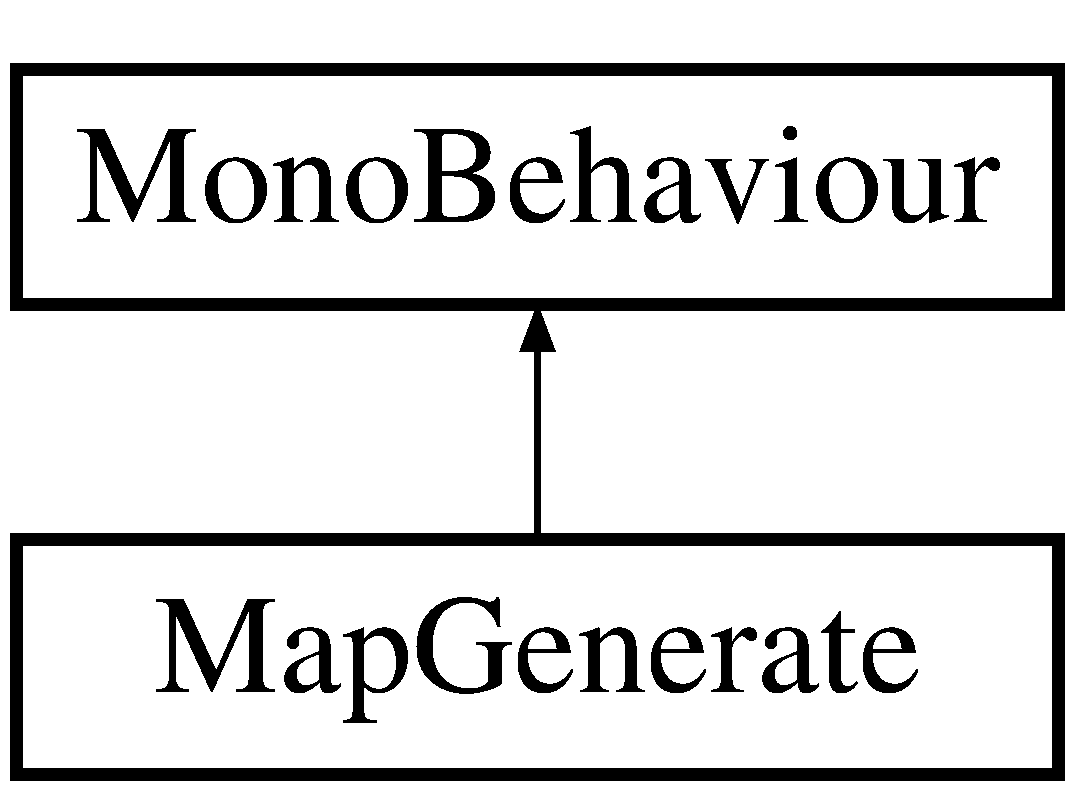
\includegraphics[height=2.000000cm]{class_map_generate}
\end{center}
\end{figure}
\subsection*{Public Attributes}
\begin{DoxyCompactItemize}
\item 
\mbox{\Hypertarget{class_map_generate_af9494468ae07d421dde634ca1f410850}\label{class_map_generate_af9494468ae07d421dde634ca1f410850}} 
Game\+Object {\bfseries tree}
\item 
\mbox{\Hypertarget{class_map_generate_a037de1b949f0bf81871d1aba4bc167b9}\label{class_map_generate_a037de1b949f0bf81871d1aba4bc167b9}} 
int {\bfseries number}
\item 
\mbox{\Hypertarget{class_map_generate_a27e7f5aeac716f9a7ba1fac63183c655}\label{class_map_generate_a27e7f5aeac716f9a7ba1fac63183c655}} 
int {\bfseries xaxis}
\item 
\mbox{\Hypertarget{class_map_generate_a8b4ca903ee45ebaf5b732f9432fa2273}\label{class_map_generate_a8b4ca903ee45ebaf5b732f9432fa2273}} 
int {\bfseries yaxis}
\item 
\mbox{\Hypertarget{class_map_generate_a373416541a633f315fdc58479ac3ab6d}\label{class_map_generate_a373416541a633f315fdc58479ac3ab6d}} 
int {\bfseries zaxis}
\end{DoxyCompactItemize}


The documentation for this class was generated from the following file\+:\begin{DoxyCompactItemize}
\item 
Assets/tree\+Generate/Map\+Generate.\+cs\end{DoxyCompactItemize}

\hypertarget{class_new_behaviour_script}{}\section{New\+Behaviour\+Script Class Reference}
\label{class_new_behaviour_script}\index{New\+Behaviour\+Script@{New\+Behaviour\+Script}}
Inheritance diagram for New\+Behaviour\+Script\+:\begin{figure}[H]
\begin{center}
\leavevmode
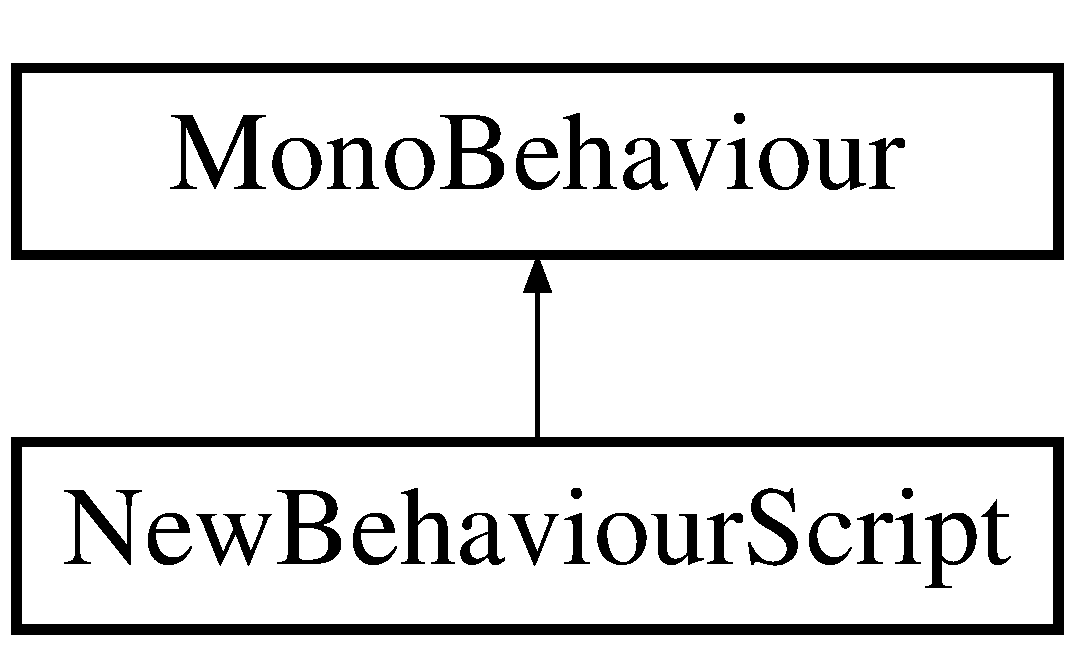
\includegraphics[height=2.000000cm]{class_new_behaviour_script}
\end{center}
\end{figure}


The documentation for this class was generated from the following file\+:\begin{DoxyCompactItemize}
\item 
Assets/scripts/bg\+Scripts/New\+Behaviour\+Script.\+cs\end{DoxyCompactItemize}

\hypertarget{classnew_game}{}\section{new\+Game Class Reference}
\label{classnew_game}\index{new\+Game@{new\+Game}}
Inheritance diagram for new\+Game\+:\begin{figure}[H]
\begin{center}
\leavevmode
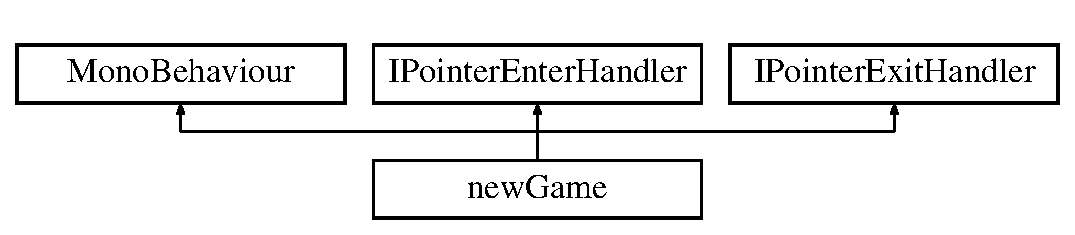
\includegraphics[height=2.000000cm]{classnew_game}
\end{center}
\end{figure}
\subsection*{Public Member Functions}
\begin{DoxyCompactItemize}
\item 
\mbox{\Hypertarget{classnew_game_aebb08e969bc2002ae3e165d6f0e1cf44}\label{classnew_game_aebb08e969bc2002ae3e165d6f0e1cf44}} 
void {\bfseries do\+New\+Game} ()
\item 
\mbox{\Hypertarget{classnew_game_a7684688306cb3bb07211cd05ad7c5998}\label{classnew_game_a7684688306cb3bb07211cd05ad7c5998}} 
void {\bfseries On\+Pointer\+Enter} (Pointer\+Event\+Data event\+Data)
\item 
\mbox{\Hypertarget{classnew_game_a7de0e1b4973147e251978f249d1c5472}\label{classnew_game_a7de0e1b4973147e251978f249d1c5472}} 
void {\bfseries On\+Pointer\+Exit} (Pointer\+Event\+Data event\+Data)
\end{DoxyCompactItemize}
\subsection*{Public Attributes}
\begin{DoxyCompactItemize}
\item 
\mbox{\Hypertarget{classnew_game_ae7bc82e056f0743b29789ee1235e0ba7}\label{classnew_game_ae7bc82e056f0743b29789ee1235e0ba7}} 
Text {\bfseries the\+Text}
\end{DoxyCompactItemize}


The documentation for this class was generated from the following file\+:\begin{DoxyCompactItemize}
\item 
Assets/scripts/buttons\+Events/new\+Game.\+cs\end{DoxyCompactItemize}

\hypertarget{class_player}{}\section{Player Class Reference}
\label{class_player}\index{Player@{Player}}
Inheritance diagram for Player\+:\begin{figure}[H]
\begin{center}
\leavevmode
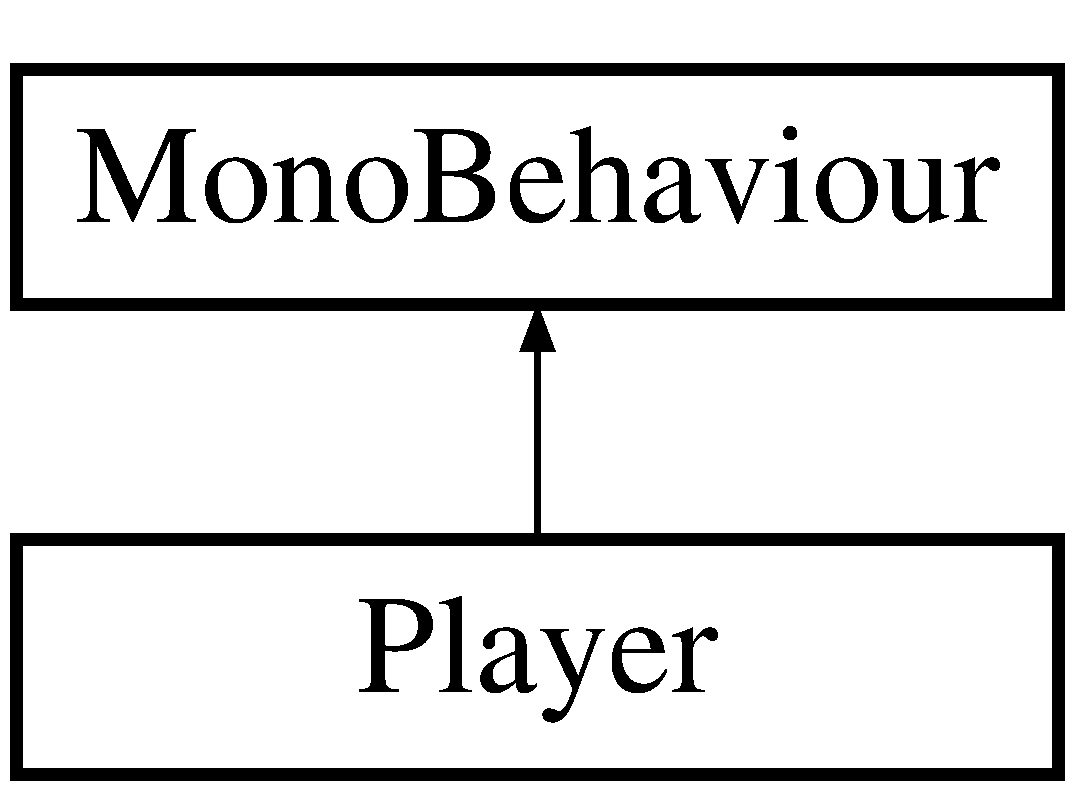
\includegraphics[height=2.000000cm]{class_player}
\end{center}
\end{figure}
\subsection*{Public Member Functions}
\begin{DoxyCompactItemize}
\item 
\mbox{\Hypertarget{class_player_a3fdebad803b97f4643696b3421be2195}\label{class_player_a3fdebad803b97f4643696b3421be2195}} 
void {\bfseries Move} ()
\item 
\mbox{\Hypertarget{class_player_aa716aeae25769b5670f983dda76932ee}\label{class_player_aa716aeae25769b5670f983dda76932ee}} 
void {\bfseries Animate\+Movement} (Vector2 direction)
\end{DoxyCompactItemize}
\subsection*{Public Attributes}
\begin{DoxyCompactItemize}
\item 
\mbox{\Hypertarget{class_player_a3224d616922f25bff5c19a70a5cee0e6}\label{class_player_a3224d616922f25bff5c19a70a5cee0e6}} 
Game\+Object {\bfseries bullet\+To\+Right}
\item 
\mbox{\Hypertarget{class_player_ad5f622aa9edaddd5838cbdce5ba76c62}\label{class_player_ad5f622aa9edaddd5838cbdce5ba76c62}} 
float {\bfseries fire\+Rate} = 0.\+5f
\item 
\mbox{\Hypertarget{class_player_af4852258f51f1596ed16923ba6613c10}\label{class_player_af4852258f51f1596ed16923ba6613c10}} 
bool {\bfseries facing\+Right} = false
\item 
\mbox{\Hypertarget{class_player_a8d784e01bdbbb7cca9d8b88cdb9815d3}\label{class_player_a8d784e01bdbbb7cca9d8b88cdb9815d3}} 
bool {\bfseries facing\+Left} = false
\end{DoxyCompactItemize}


The documentation for this class was generated from the following file\+:\begin{DoxyCompactItemize}
\item 
Assets/scripts/player/Player.\+cs\end{DoxyCompactItemize}

\hypertarget{class_rabbit}{}\section{Rabbit Class Reference}
\label{class_rabbit}\index{Rabbit@{Rabbit}}
Inheritance diagram for Rabbit\+:\begin{figure}[H]
\begin{center}
\leavevmode
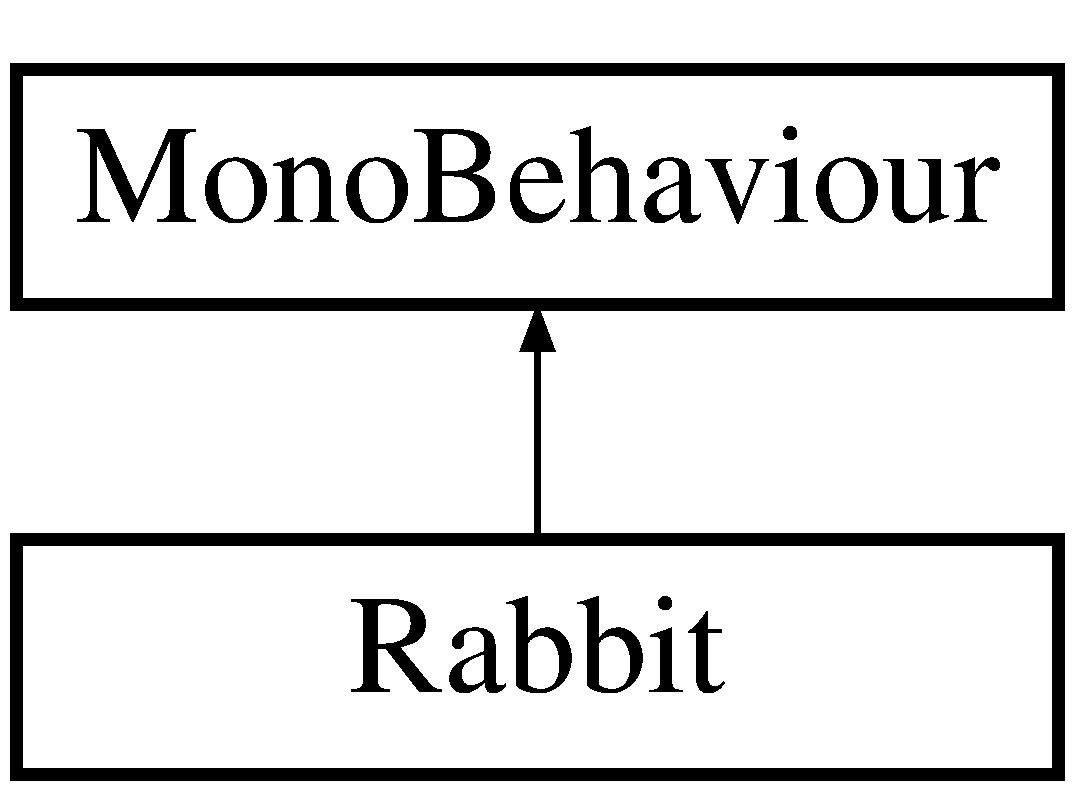
\includegraphics[height=2.000000cm]{class_rabbit}
\end{center}
\end{figure}


The documentation for this class was generated from the following file\+:\begin{DoxyCompactItemize}
\item 
Assets/scripts/rabbit/Rabbit.\+cs\end{DoxyCompactItemize}

\hypertarget{classrabbit}{}\section{rabbit Class Reference}
\label{classrabbit}\index{rabbit@{rabbit}}
Inheritance diagram for rabbit\+:\begin{figure}[H]
\begin{center}
\leavevmode
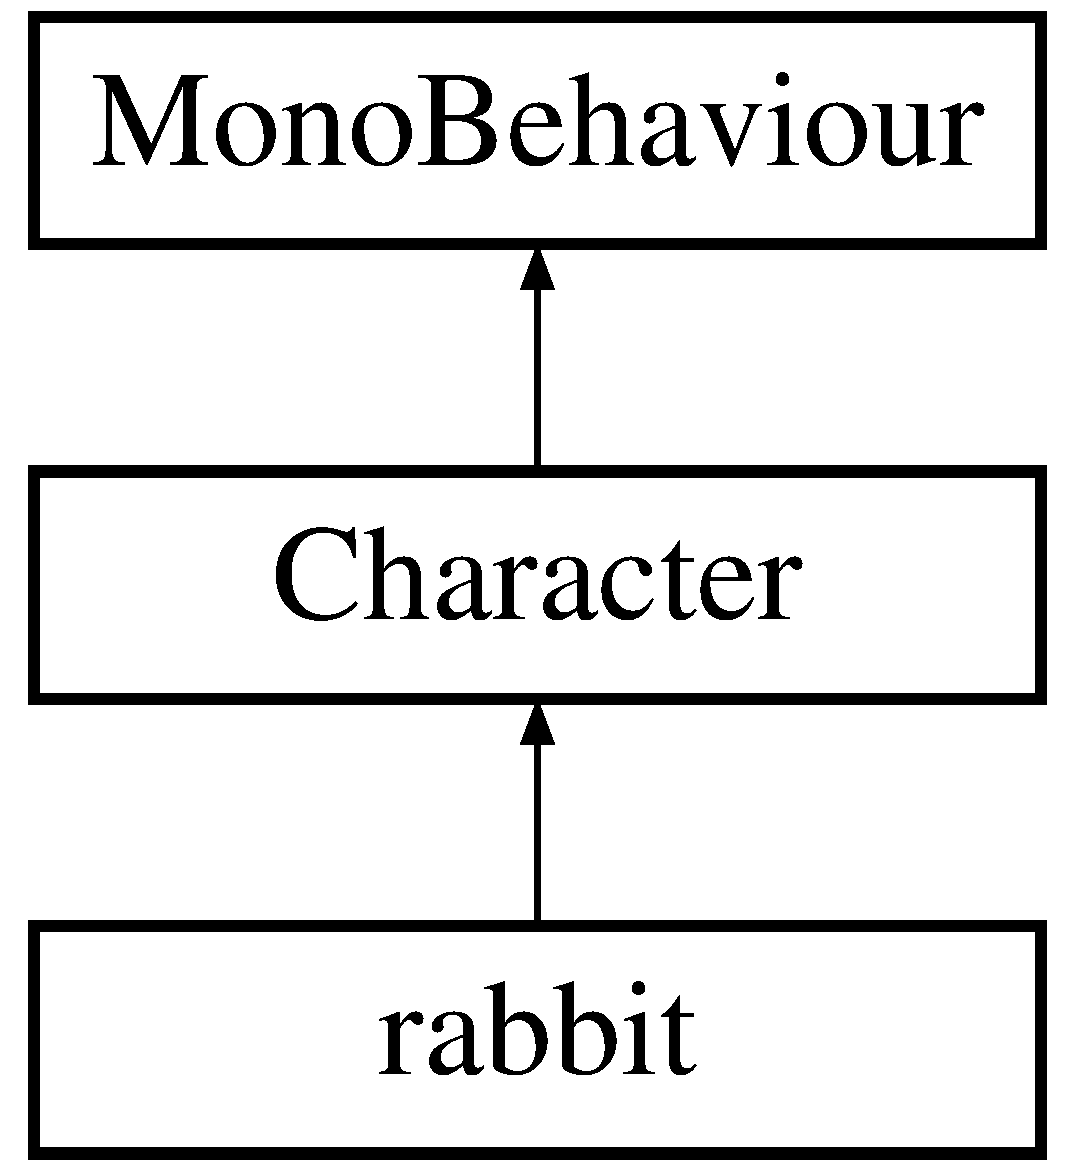
\includegraphics[height=3.000000cm]{classrabbit}
\end{center}
\end{figure}
\subsection*{Public Attributes}
\begin{DoxyCompactItemize}
\item 
\mbox{\Hypertarget{classrabbit_a3eafc8ac14d015793b30ddf3f987f460}\label{classrabbit_a3eafc8ac14d015793b30ddf3f987f460}} 
int {\bfseries move\+Speed}
\item 
\mbox{\Hypertarget{classrabbit_adbee5f933d949500c6cdeac98139a5f4}\label{classrabbit_adbee5f933d949500c6cdeac98139a5f4}} 
int {\bfseries rotation\+Speed}
\end{DoxyCompactItemize}
\subsection*{Properties}
\begin{DoxyCompactItemize}
\item 
\mbox{\Hypertarget{classrabbit_a69598d517f6349f2e88008cf10ee304f}\label{classrabbit_a69598d517f6349f2e88008cf10ee304f}} 
Transform {\bfseries Target}\hspace{0.3cm}{\ttfamily  \mbox{[}get, set\mbox{]}}
\end{DoxyCompactItemize}
\subsection*{Additional Inherited Members}


The documentation for this class was generated from the following file\+:\begin{DoxyCompactItemize}
\item 
Assets/rabbit.\+cs\end{DoxyCompactItemize}

\hypertarget{classrange}{}\section{range Class Reference}
\label{classrange}\index{range@{range}}
Inheritance diagram for range\+:\begin{figure}[H]
\begin{center}
\leavevmode
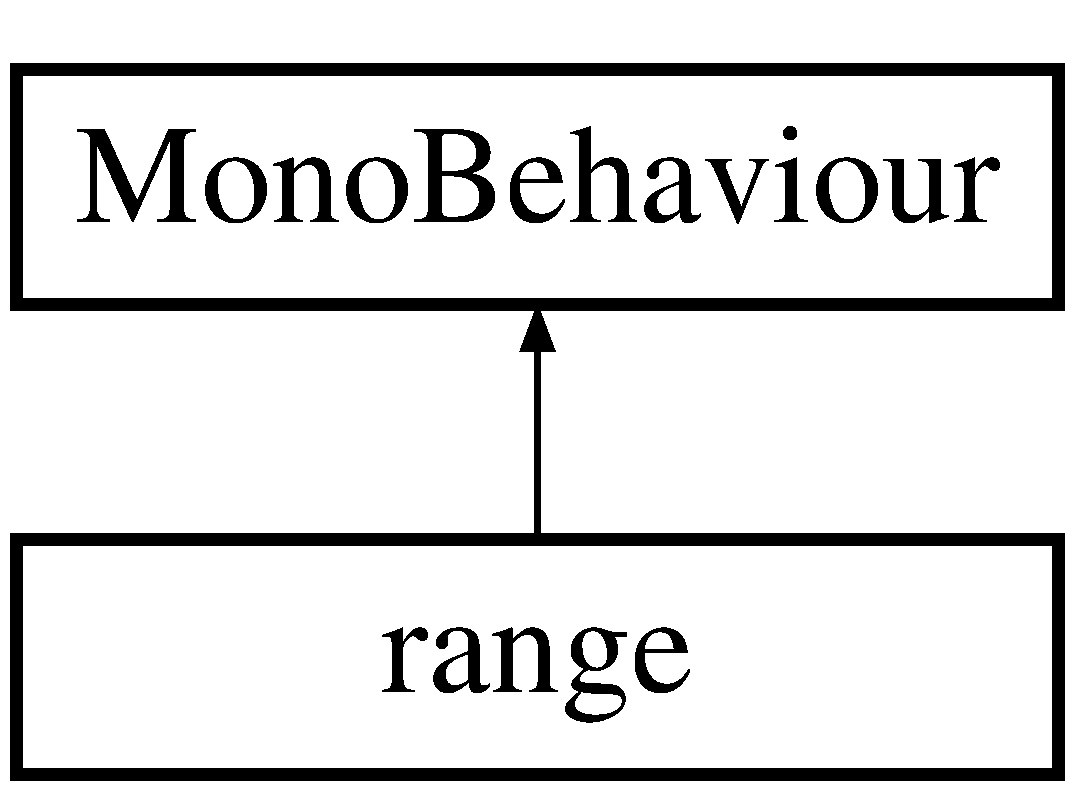
\includegraphics[height=2.000000cm]{classrange}
\end{center}
\end{figure}


The documentation for this class was generated from the following file\+:\begin{DoxyCompactItemize}
\item 
Assets/range.\+cs\end{DoxyCompactItemize}

\hypertarget{class_range}{}\section{Range Class Reference}
\label{class_range}\index{Range@{Range}}
Inheritance diagram for Range\+:\begin{figure}[H]
\begin{center}
\leavevmode
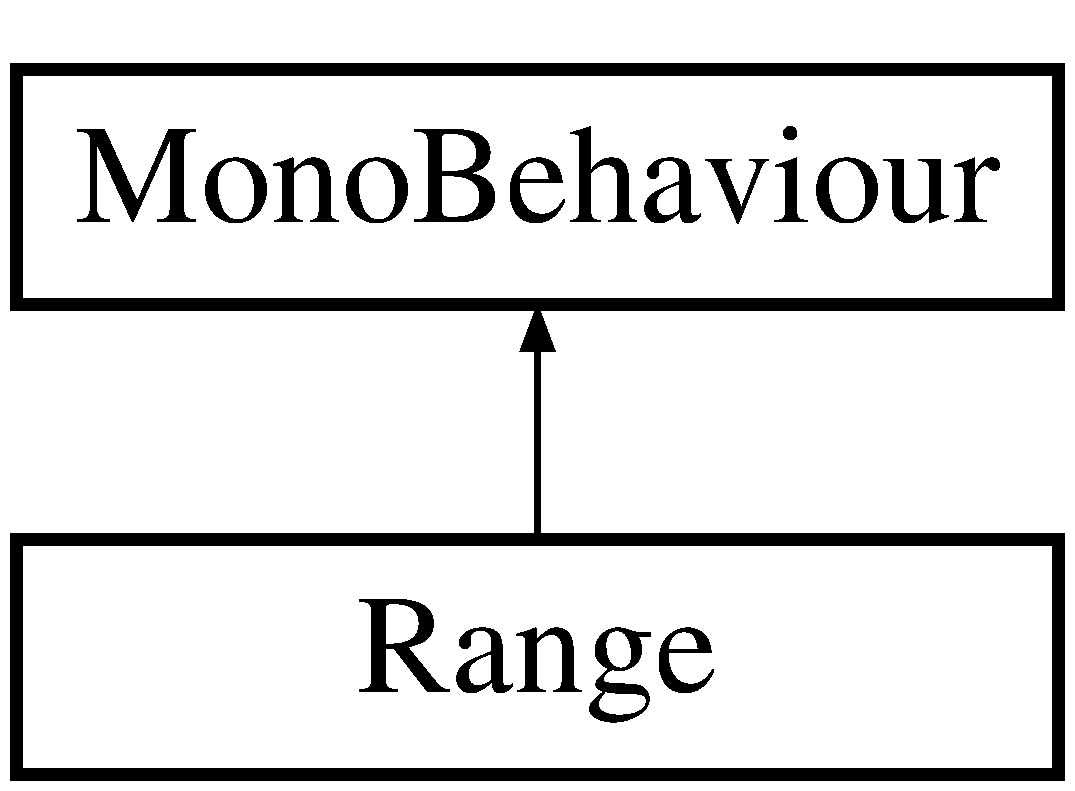
\includegraphics[height=2.000000cm]{class_range}
\end{center}
\end{figure}


The documentation for this class was generated from the following file\+:\begin{DoxyCompactItemize}
\item 
Assets/scripts/wolf/Range.\+cs\end{DoxyCompactItemize}

\hypertarget{classsave_btn}{}\section{save\+Btn Class Reference}
\label{classsave_btn}\index{save\+Btn@{save\+Btn}}
Inheritance diagram for save\+Btn\+:\begin{figure}[H]
\begin{center}
\leavevmode
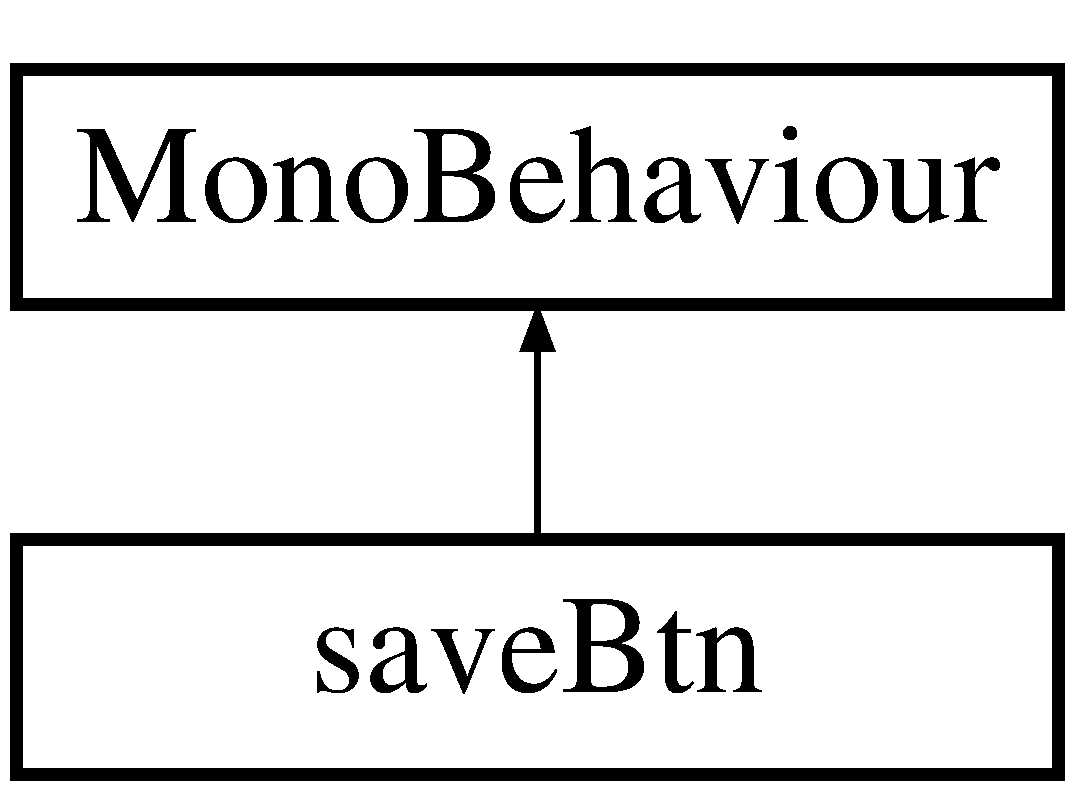
\includegraphics[height=2.000000cm]{classsave_btn}
\end{center}
\end{figure}
\subsection*{Public Member Functions}
\begin{DoxyCompactItemize}
\item 
\mbox{\Hypertarget{classsave_btn_a0e4102d46dfe26be5bc4d74726365989}\label{classsave_btn_a0e4102d46dfe26be5bc4d74726365989}} 
void {\bfseries Save} ()
\end{DoxyCompactItemize}


The documentation for this class was generated from the following file\+:\begin{DoxyCompactItemize}
\item 
Assets/scripts/buttons\+Events/save\+Btn.\+cs\end{DoxyCompactItemize}

\hypertarget{class_shooting}{}\section{Shooting Class Reference}
\label{class_shooting}\index{Shooting@{Shooting}}
Inheritance diagram for Shooting\+:\begin{figure}[H]
\begin{center}
\leavevmode
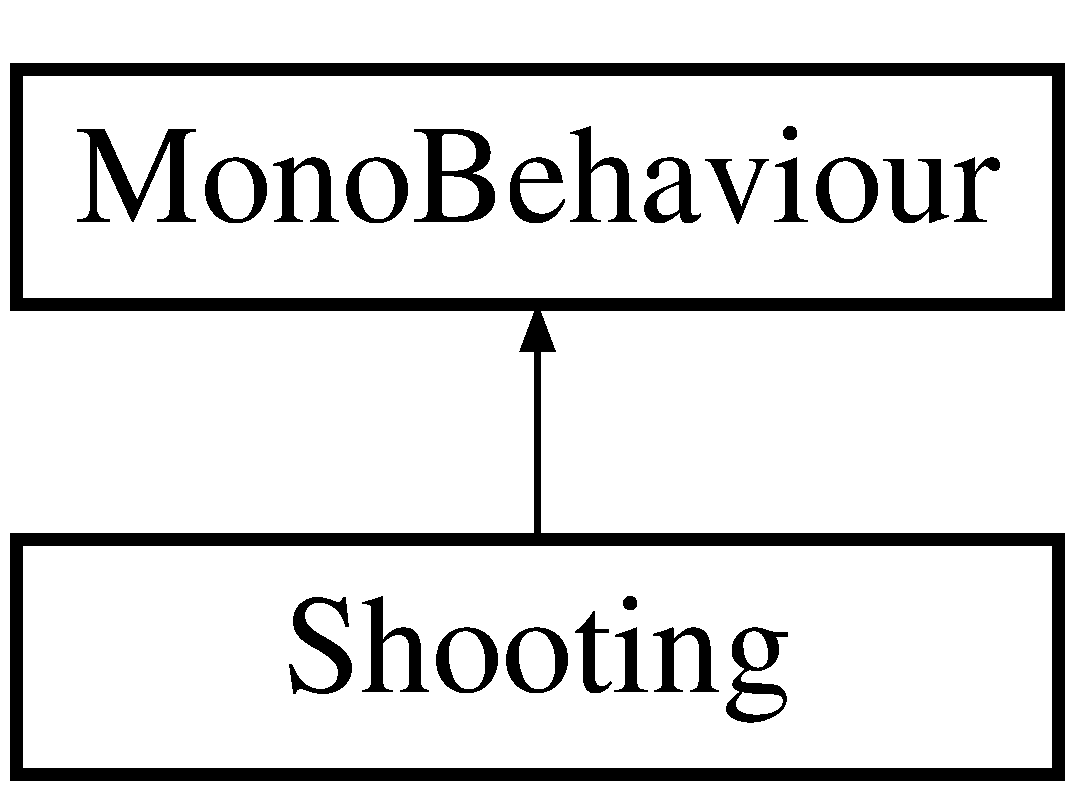
\includegraphics[height=2.000000cm]{class_shooting}
\end{center}
\end{figure}
\subsection*{Public Attributes}
\begin{DoxyCompactItemize}
\item 
\mbox{\Hypertarget{class_shooting_a332399d24695a92949c8d5bbac43d26c}\label{class_shooting_a332399d24695a92949c8d5bbac43d26c}} 
Game\+Object {\bfseries bullet}
\end{DoxyCompactItemize}


The documentation for this class was generated from the following file\+:\begin{DoxyCompactItemize}
\item 
Assets/scripts/Shooting.\+cs\end{DoxyCompactItemize}

\hypertarget{class_simply_player_behaviour}{}\section{Simply\+Player\+Behaviour Class Reference}
\label{class_simply_player_behaviour}\index{Simply\+Player\+Behaviour@{Simply\+Player\+Behaviour}}
Inheritance diagram for Simply\+Player\+Behaviour\+:\begin{figure}[H]
\begin{center}
\leavevmode
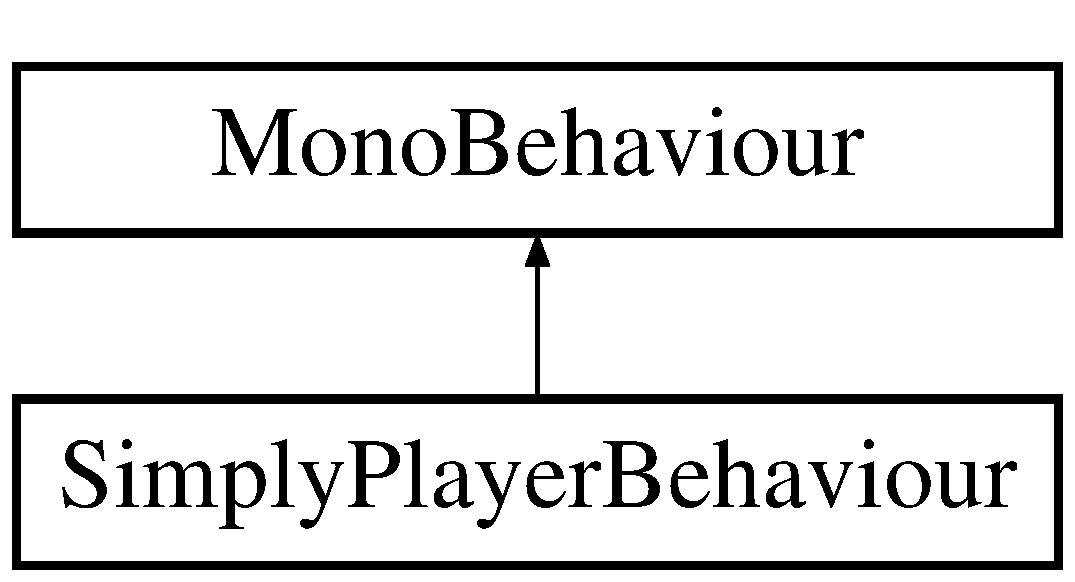
\includegraphics[height=2.000000cm]{class_simply_player_behaviour}
\end{center}
\end{figure}


The documentation for this class was generated from the following file\+:\begin{DoxyCompactItemize}
\item 
Assets/scripts/bg\+Scripts/Simply\+Player\+Behaviour.\+cs\end{DoxyCompactItemize}

\hypertarget{class_wolf}{}\section{Wolf Class Reference}
\label{class_wolf}\index{Wolf@{Wolf}}
Inheritance diagram for Wolf\+:\begin{figure}[H]
\begin{center}
\leavevmode
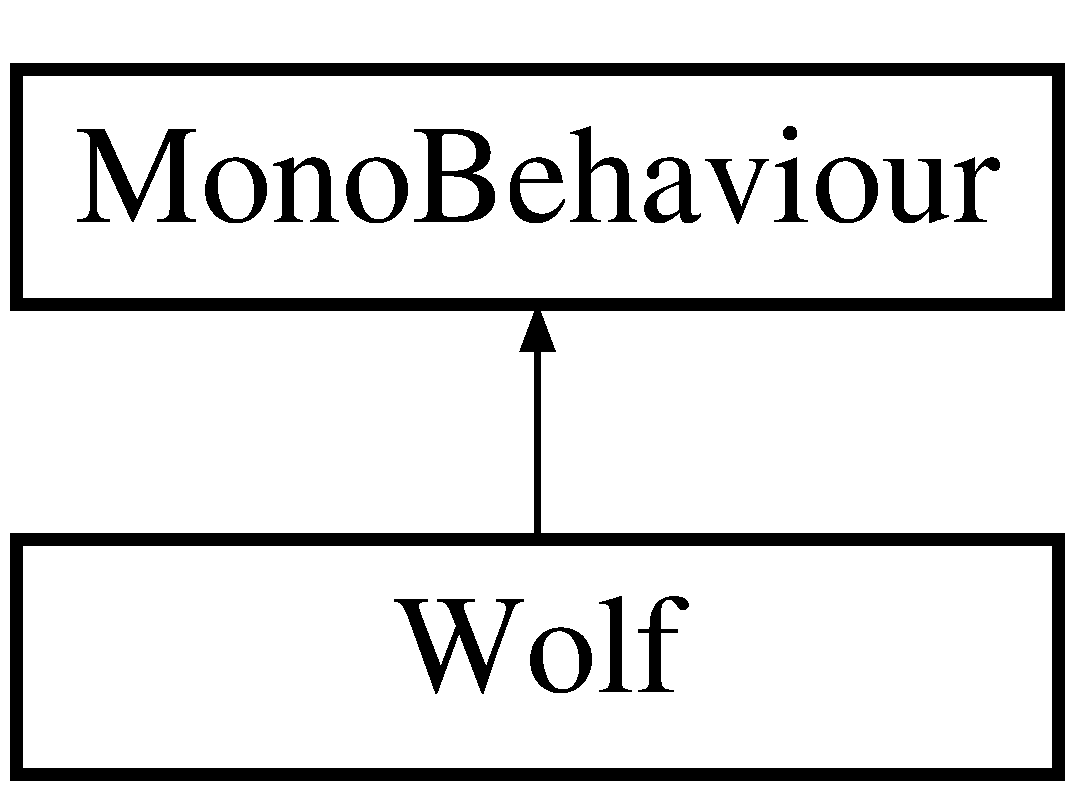
\includegraphics[height=2.000000cm]{class_wolf}
\end{center}
\end{figure}


The documentation for this class was generated from the following file\+:\begin{DoxyCompactItemize}
\item 
Assets/scripts/wolf/Wolf.\+cs\end{DoxyCompactItemize}

\hypertarget{class_zdrowie_u_i}{}\section{Zdrowie\+UI Class Reference}
\label{class_zdrowie_u_i}\index{Zdrowie\+UI@{Zdrowie\+UI}}
Inheritance diagram for Zdrowie\+UI\+:\begin{figure}[H]
\begin{center}
\leavevmode
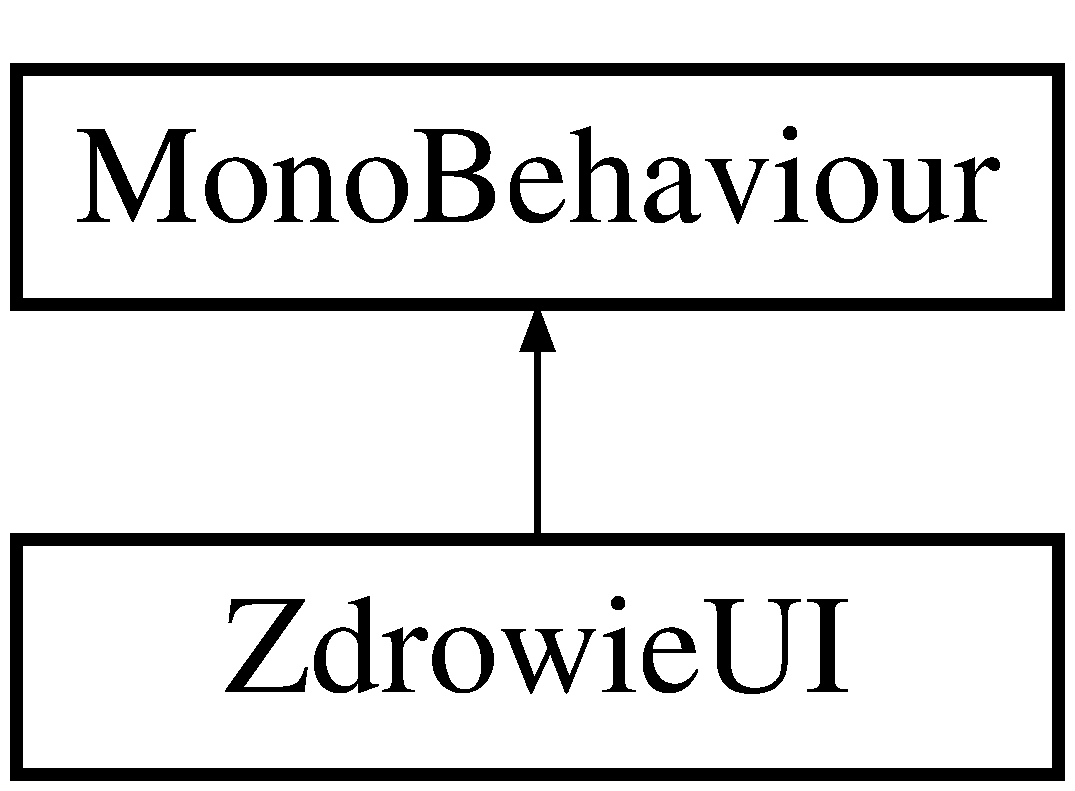
\includegraphics[height=2.000000cm]{class_zdrowie_u_i}
\end{center}
\end{figure}
\subsection*{Public Attributes}
\begin{DoxyCompactItemize}
\item 
\mbox{\Hypertarget{class_zdrowie_u_i_a8830091d8a564921bfbe90ffeee3c137}\label{class_zdrowie_u_i_a8830091d8a564921bfbe90ffeee3c137}} 
G\+U\+I\+Skin {\bfseries skin}
\end{DoxyCompactItemize}


The documentation for this class was generated from the following file\+:\begin{DoxyCompactItemize}
\item 
Assets/scripts/zdrowie/Zdrowie\+U\+I.\+cs\end{DoxyCompactItemize}

%--- End generated contents ---

% Index
\backmatter
\newpage
\phantomsection
\clearemptydoublepage
\addcontentsline{toc}{chapter}{Index}
\printindex

\end{document}
